\documentclass{beamer}
\usetheme{metropolis}
\usepackage{mymathstyle}
\usepackage{subcaption}
\usefonttheme[onlymath]{serif}

\newcommand{\softreliprod}[3]{\left\langle #1, #2 \, \vert \, #3 \right\rangle_\mathrm{rel}}
\newcommand{\reliprod}[2]{\left\langle #1, #2 \right\rangle_\mathrm{rel}}
% \let\phi\varphi

\AtBeginSection[]
{
  \begin{frame}
    \frametitle{Table of Contents}
    \tableofcontents[currentsection]
  \end{frame}
}
\setcounter{tocdepth}{1}


\title{Relational convolutional networks: \\\small{A framework for learning representations of hierarchical relations}}
\date{\today}

\begin{document}

\frame{\titlepage}

\begin{frame}{Outline}
    % set depth to 1
    \tableofcontents
\end{frame}

\section{Motivation}
\begin{frame}{Motivation}
\begin{itemize}
    \item Research into relational representation learning has uncovered effective inductive biases
    \item A key to the power of deep representation learning is compositionality (e.g., CNNs, FFNNs, Transformers, etc.)
    \item So far, relational architectures have been ``flat,'' w/o explicit support for learning hierarchical relations
  \end{itemize}
  \center{
    \textit{Can we develop a compositional framework for learning representations of hierarchical relations?}
  }
\end{frame}

\section{High-level idea}

\begin{frame}{High-level idea of architecture}
  \begin{figure}
    \centering
    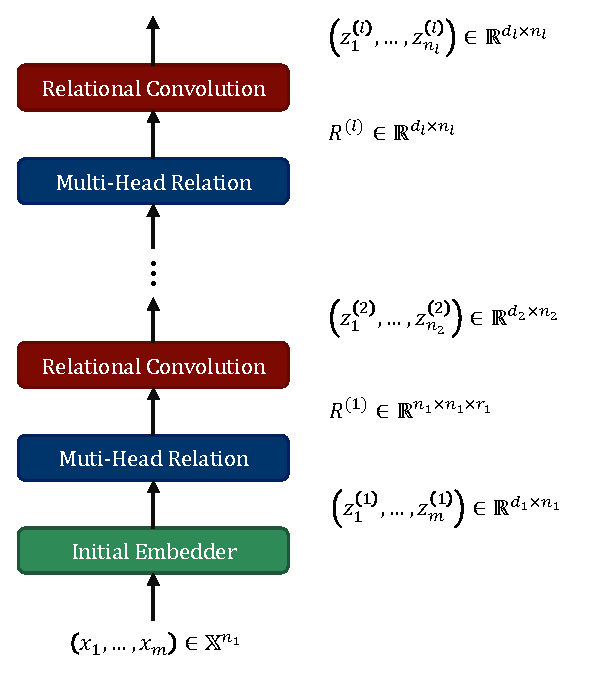
\includegraphics[height=0.8\textheight]{figs/relconv_architecture.pdf}
  \end{figure}
\end{frame}

\section{Multi-Dimensional Inner-Product Relations}
\begin{frame}{Multi-Dimensional  Inner Product Relations}
  Informed by previous work on relational representation, we model relations as inner products between feature maps,
  \begin{equation*}%\label{eq:relation_function}
    r(x, y) = \begin{pmatrix}
        \iprod{\phi_1(x)}{\psi_1(y)} \\ \vdots \\ \iprod{\phi_{d_r}(x)}{\psi_{d_r}(y)}
      \end{pmatrix} \in \reals^{d_r},
\end{equation*}

The ``relation tensor,'' is the set of all pairwise relations, $R \in \reals^{m \times m \times d_r},\ R[i,j] = r(x_i, x_j)$.
\end{frame}

\section{Relational convolutions}
\begin{frame}{Relational convolutions: Idea}
  High-level idea: consider groups of objects, and model the relational pattern within the group.

  Learn ``graphlet filters,'' which represent a template of relations against which relations within groups are compared.
\end{frame}


\begin{frame}{Relational convolutions: preview}
  \begin{figure}
    \centering
    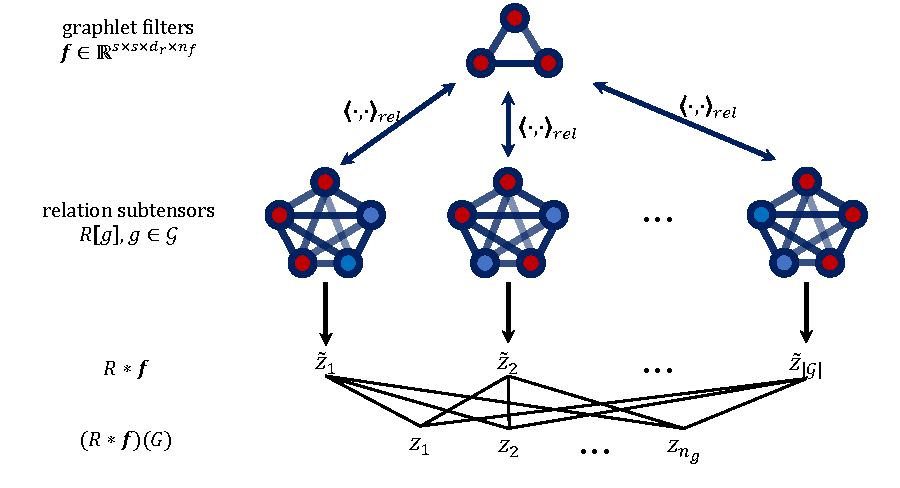
\includegraphics[width=\textwidth]{figs/relconv_diagram2.pdf}
  \end{figure}
\end{frame}

\begin{frame}{Relational convolutions: graphlet filters and the relational inner product}
  $f_1 \in \reals^{s \times s \times d_r}$ is a ``graphlet filter'' with filter size $s$. $g$ is a subset of the objects to consider. $\bm{f} = (f_1, \ldots, f_{n_f}) \in \reals^{s \times s \times d_r \times n_f}$ is a collection of graphlet fiters.

  \begin{equation*}% \label{eq:relational_inner_prod_one_filt}
    \reliprod{R[g]}{f_1} \coloneqq \sum_{i,j \in g} \iprod{R[i,j]}{f_1[i,j]}_{\reals^{d_r}} = \sum_{i,j \in g} \sum_{k \in [d_r]} R[i,j,k] f_1[i,j,k].
  \end{equation*}

  \begin{equation*}
    % \label{eq:relational_inner_prod}
    \reliprod{R[g]}{\bm{f}} \coloneq \begin{pmatrix} \reliprod{R[g]}{f_1} \\ \vdots 
    \\ \reliprod{R[g]}{f_{n_f}} \end{pmatrix} \in \mathbb{R}^{n_f}.
  \end{equation*}
\end{frame}

\begin{frame}{Aside: symmetric variant of relational inner product}
  Sometimes, it may be useful to have symmetry across permutations of $g$ as an inductive bias. This can be achieved with pooling over permutations.
  \begin{equation*}%\label{eq:symmetric_relational_inner_prod}
    \iprod{R[g]}{\bm{f}}_{\mathrm{rel}, \mathrm{sym}} \coloneq \mathrm{Pool}\paren{\set{\reliprod{R[g']}{\bm{f}} \colon g' \in g!}},
  \end{equation*}
\end{frame}

\begin{frame}{Putting it together: the convolution}
  The ``relational convolution,'' is the set of relational inner products with a series of groups $g \in \calG$,
  \begin{equation*}
    % \label{eq:relational_convolution}
    R \ast \bm{f} \coloneq \left( \reliprod{R[g]}{\boldsymbol{f}} \right)_{g \in \calG} \equiv \left(z_1, ..., z_{\abs{\calG}}\right) \in (\mathbb{R}^{n_f})^{\abs{\calG}}
\end{equation*}

This produces a sequence of objects, each of which summarizes the relational pattern within some set of objects.
\end{frame}

\begin{frame}{Relational convolution with ``soft'' groups: the idea}
  If the relevant set of groupings $\calG$ is known a priori: great!

  Often times, this won't be known, and we'd like to \textit{learn} the relevant groupings to consider.

  To do this, we need to formalize a notion of relational convolutions with ``soft groups,'' that may be produced be some other component of the model.

  Suppose we are given a ``group matrix,'' $G \in \reals^{m \times n_g}$, where $n_g$ is \# of groups and $G[i, k]$ represents degree to which object $i \in [m]$ belongs to group $k \in [n_g]$.
\end{frame}

\begin{frame}{Relational convolution with ``soft'' groups}
  \begin{equation*}%\label{eq:group_match_score}
    \begin{split}
        G &\gets \text{SoftPlus}(G)\\
        \alpha_{gk} &\gets \text{Normalize}\paren{\bra{\prod_{i \in g} G[i,k]}_{g \in \calG}}, \quad g \in \calG, k \in [n_g],
    \end{split}
  \end{equation*}

  \begin{equation*}%\label{eq:soft_relational_inner_prod}
    \langle R, \boldsymbol{f} \, \vert \, G_k \rangle_R \coloneqq \sum_{g \in \calG} \alpha_{gk} \iprod{R[g]}{\boldsymbol{f}}_\mathrm{rel}.
  \end{equation*}

  \begin{equation*}%\label{eq:soft_relational_convolution_groups}
    (R \ast \bm{f})(G) = \left( \softreliprod{R}{\bm{f}}{G_1}, \ldots, \softreliprod{R}{\bm{f}}{G_{n_g}} \right) \in \left(\mathbb{R}^{n_f}\right)^{n_g}.
  \end{equation*}
\end{frame}

\section{Grouping layers}
\begin{frame}{Grouping layers}
\center{
  \textit{Okay, but how do we get $G$? How do we get a model to identify the relevant groups that it should consider?}
}
\end{frame}

\begin{frame}{Grouping layers: some ideas}
  Depending on the underlying task, we propose a few ways to model groups of objects.
  \begin{enumerate}
    \item Group objects based on the temporal (positional) order that they appear in the sequence
    \item Group objects based on their features
    \item Group objects based on their own features as well as the context in which they appear.
  \end{enumerate}
\end{frame}

\begin{frame}{Grouping layers}
  \textbf{Temporal (positional) grouping} Learn $G \in \reals^{m \times n_g}$ directly as a parameter of the model.

  \textbf{Feature-based grouping} Learn a mapping (e.g., MLP) from features to group membership vectors
  \begin{equation}\label{eq:feat_grouping}
    G \gets \begin{bmatrix}
        \phi(1, x_1)^\top \\
        \vdots \\
        \phi(m, x_m)^\top
    \end{bmatrix} \in \reals^{m \times n_g},
\end{equation}
\end{frame}

\begin{frame}{Grouping layers}
\textbf{Contextual grouping} Perform message-passing first to incorporate information about the object's context, then map that to a group vector.
\begin{equation}\label{eq:context_grouping}
  \begin{split}
      E_i &\gets \mathrm{MessagePassing}\paren{x_i, \set{x_1, \ldots, x_m}}, \ i \in [m] \\
      G &\gets \begin{bmatrix}\mathrm{MLP}(E_1)^\top \\ \vdots \\ \mathrm{MLP}(E_m)^\top \end{bmatrix} \in \reals^{m \times n_g}.
  \end{split}
\end{equation}
\end{frame}


\begin{frame}{Relational convolutions}
  \begin{figure}
    \centering
    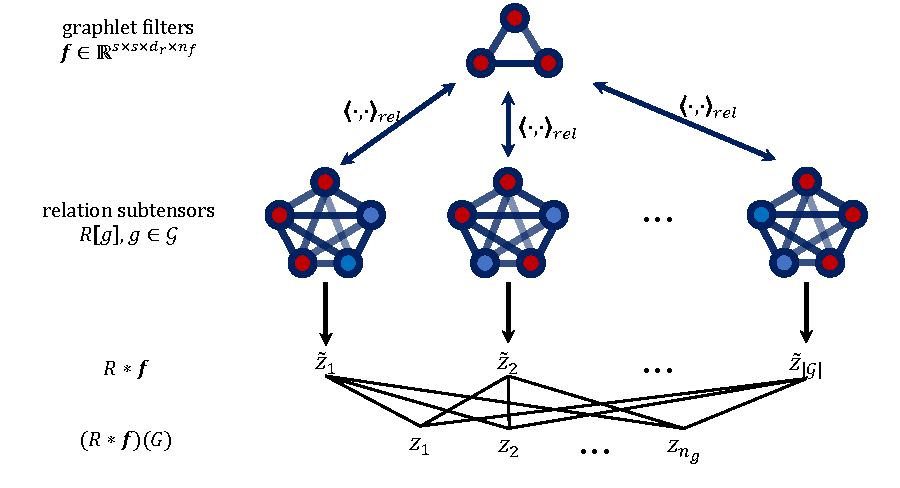
\includegraphics[width=\textwidth]{figs/relconv_diagram2.pdf}
  \end{figure}
\end{frame}

\begin{frame}{Architecture}
  \begin{figure}
    \centering
    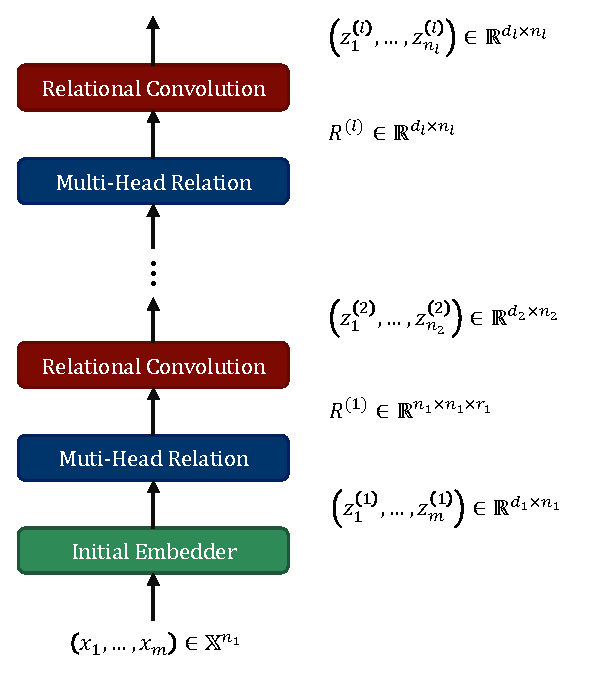
\includegraphics[height=0.8\textheight]{figs/relconv_architecture.pdf}
  \end{figure}
\end{frame}

\section{Experiments}
\subsection{Relational games}
\begin{frame}{Relational games tasks}
  \begin{figure}
    \centering
    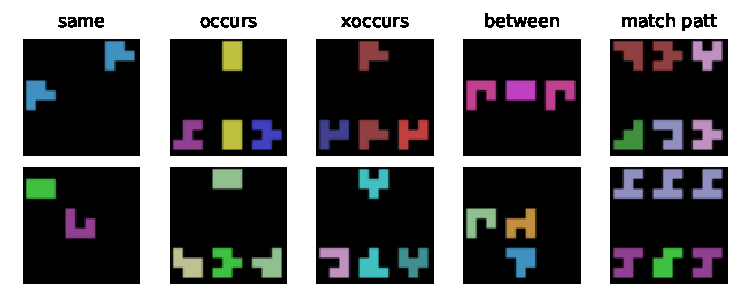
\includegraphics[width=\textwidth]{figs/relational_games_tasks.pdf}
  \end{figure}
\end{frame}
\begin{frame}{Relational games objects}
  \begin{figure}
    \centering
    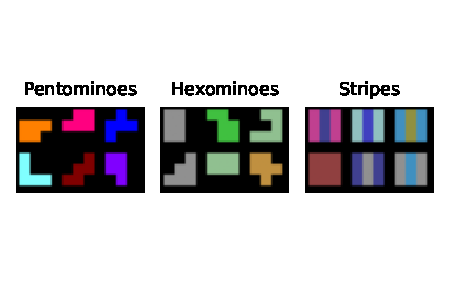
\includegraphics[width=0.8\textwidth]{figs/relational_games_objects.pdf}
  \end{figure}
\end{frame}

\begin{frame}{Out-of-Distribution Generalization}
  \begin{figure}
    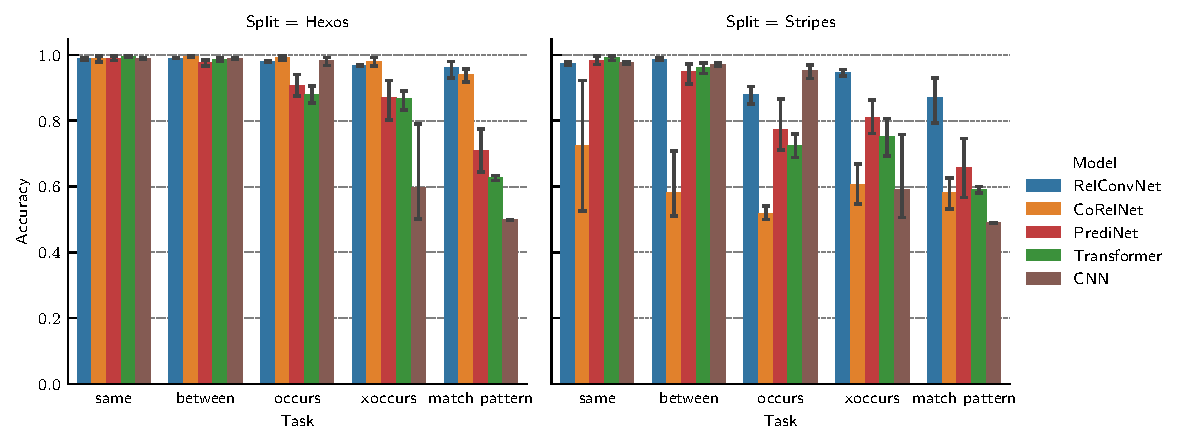
\includegraphics[width=1.1\textwidth]{figs/experiments/relgames_ood_acc.pdf}
  \end{figure}
\end{frame}

\subsection{Contains "SET"}
\begin{frame}{Contains "SET"}
  \begin{figure}
    \centering
    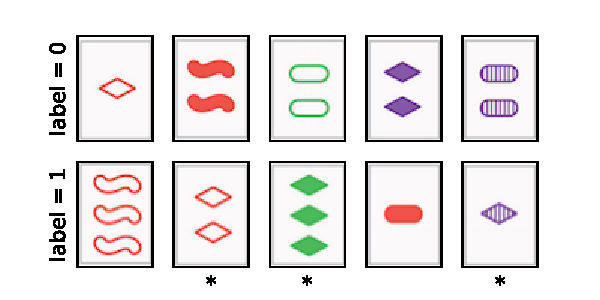
\includegraphics[width=0.8\textwidth]{figs/contains_set_example.pdf}
  \end{figure}
\end{frame}

\begin{frame}{Contains "SET": Generalization accuracy}
  \begin{figure}
    \centering
    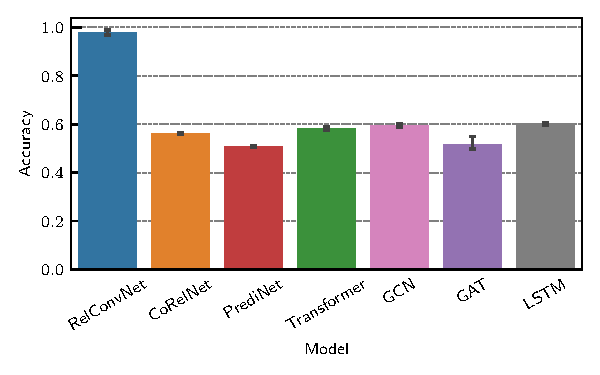
\includegraphics[width=0.8\textwidth]{figs/experiments/contains_set_acc.pdf}
  \end{figure}
\end{frame}

\begin{frame}{Contains "SET": Training curves}
  \begin{figure}
    \centering
    \begin{subfigure}{0.49\textwidth}
      \centering
      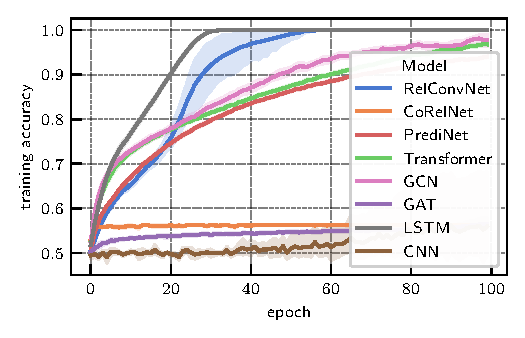
\includegraphics[width=\textwidth]{figs/experiments/contains_set_training_curves_trainacc.pdf}
    \end{subfigure}
    \begin{subfigure}{0.49\textwidth}
      \centering
      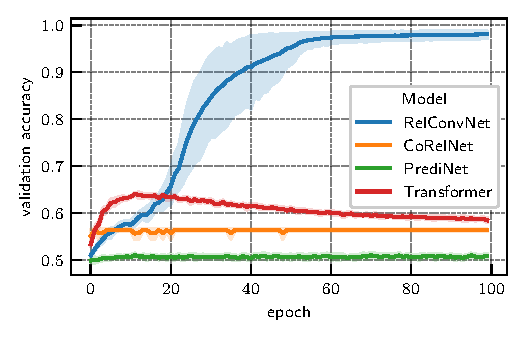
\includegraphics[width=\textwidth]{figs/experiments/contains_set_training_curves_valacc.pdf}
    \end{subfigure}
  \end{figure}
\end{frame}

% \begin{frame}{}
%   \begin{figure*}
%     \includegraphics{figs/experiments}
%   \end{figure*}
% \end{frame}

\section{Representational geometry}

\begin{frame}{Representations learned by encoders of MD-IPR}
  \begin{figure}
    \centering
    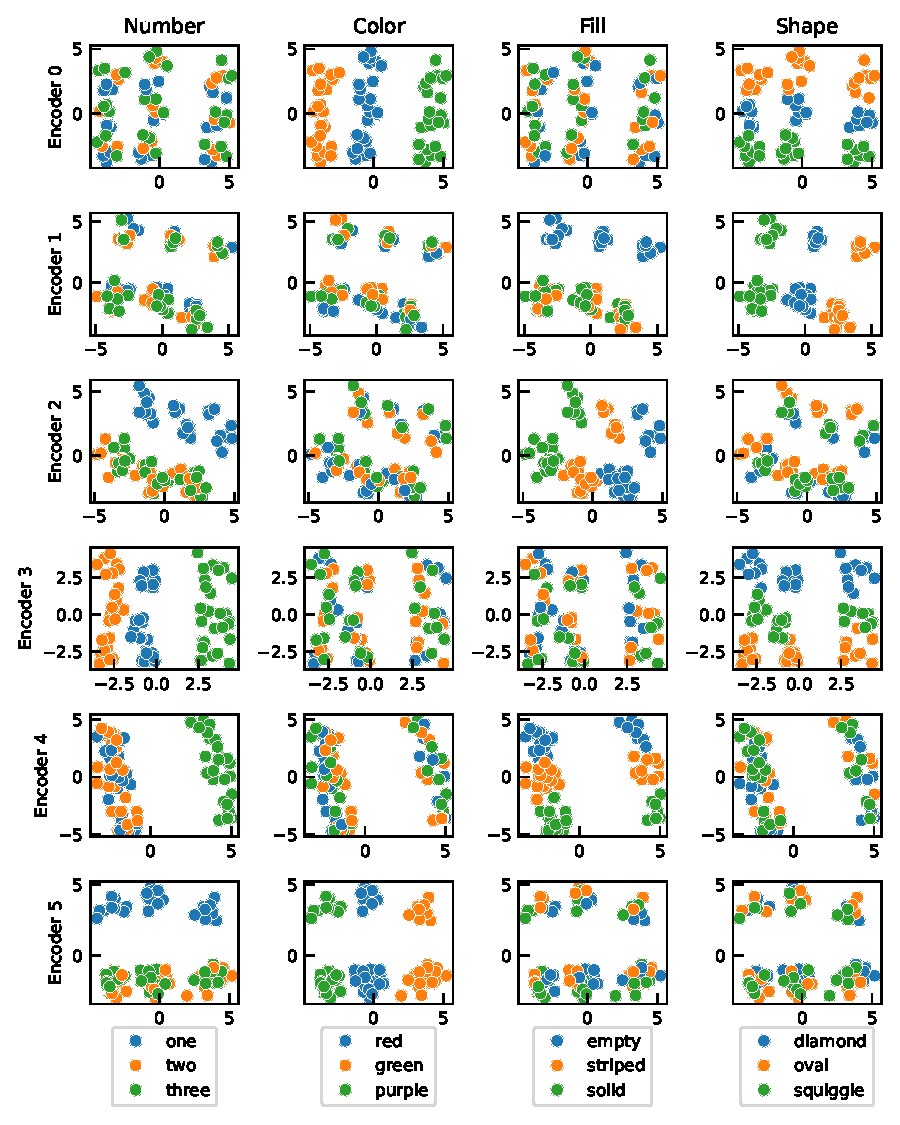
\includegraphics[height=0.9\textheight]{figs/representation_analysis/mdipr_encoders_rep.pdf}
  \end{figure}
\end{frame}

\begin{frame}{Geometry of MD-IPR relations}
  \begin{figure}
    \centering
    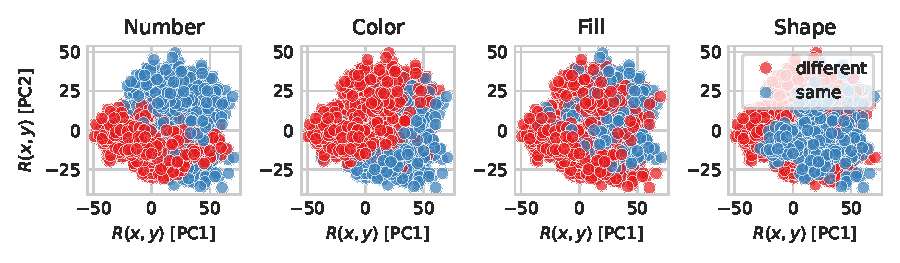
\includegraphics[width=\textwidth]{figs/representation_analysis/mdipr_rel_rep.pdf}
  \end{figure}
\end{frame}

\begin{frame}{Geometry of relational convolutions}
  \begin{figure}
    \centering
    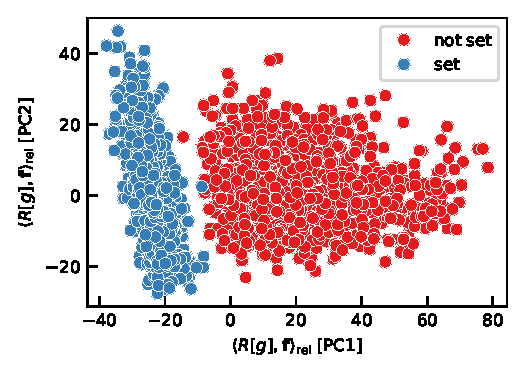
\includegraphics[width=\textwidth]{figs/representation_analysis/conv_rep.pdf}
  \end{figure}
\end{frame}

\end{document}
